\documentclass[a4paper]{book}
\usepackage[utf8]{inputenc}
\usepackage[margin=3cm]{geometry} % For smaller margins
\usepackage{appendix} % For appendix support
\usepackage{tikz, pgfplots} % For the skill outcome graph
    \pgfplotsset{width = \textwidth, compat = newest}
\usepackage{graphicx} % For advanced picture insertion
\usepackage{pdfpages} % For inserting PDFs
\usepackage{multicol} % For supporting multi-columnar tables
\usepackage{tcolorbox} % For coloured info boxes
    \tcbuselibrary{skins}
    \tcbset{colback=brown!10, fonttitle=\scshape}
\usepackage{textcomp} % For the interrobang
\usepackage[sc,sf,bf]{titlesec} % for custom titles
\usepackage{sectsty} % for section styles
\usepackage{fancyhdr} % for "fancy" headers
\usepackage[notmath]{sansmathfonts} % for a sans-serif small-caps font
\usepackage{enumitem} % for finer control over enumerations
 
\usepackage{epsdice}

%%%%%%%%%%%%%%%%%%%%%%%%%%%%%%%%%
%% CHAPTERS & SECTION HEADINGS %%
%%%%%%%%%%%%%%%%%%%%%%%%%%%%%%%%%


% Simplifies chapter titles
% No longer says
% Chapter 2
% Game Creation
% but instead simply
% 2 Game Creation
\titleformat{\chapter}[hang]
{\sffamily\bfseries\scshape\Huge}
{\thechapter\quad}{0pt}{}{}

% Removes unnecessarily large margin above chapter title
\titlespacing*{\chapter}{0pt}{-\topskip}{40pt}

% Set the remaining titles to be sans serif and small caps
\allsectionsfont{\sffamily\scshape}

%%%%%%%%%%%%%%%%%
%% THUMB INDEX %%
%%%%%%%%%%%%%%%%%

\renewcommand{\chaptermark}[1]{\markboth{\textsc{\thechapter\ #1}}{}}

%%%%%%%%%%%%%%%%%%%%%%%
%% CUSTOM TEXT BOXES %%
%%%%%%%%%%%%%%%%%%%%%%%
\newtcolorbox{note}{
    enhanced, % enable advanced settings
    left = 10mm, % pushes text away from the left edge by 10mm
    sharp corners, % disables rounded corners
    rounded corners = southeast, % "round" the bottom right corner
    arc is angular, % make the "round" corner an angle
    arc = 3mm, % controls corner cut
    boxrule=0.6pt, % sets box line thickness
    underlay={%
        \path[fill=tcbcolback!80!black] ([yshift=3mm]interior.south east)--++(-0.4,-0.1)--++(0.1,-0.2); % triangle
        \path[draw=tcbcolframe,shorten <=-0.05mm,shorten >=-0.05mm] ([yshift=3mm]interior.south east)--++(-0.4,-0.1)--++(0.1,-0.2); % triangle edge
        \path[fill=gray!50!black,draw=none] (interior.south west) rectangle node[brown!10]{\Huge\bfseries \textinterrobang} ([xshift=8mm]interior.north west);
    },
    drop fuzzy shadow % adds drop shadow
}

\newtcolorbox{example}{
    enhanced,
    title = Example,
    before upper={\parindent15pt\noindent} % add paragraph indentation
}

\begin{document}

\begin{titlepage}
\begin{center}
    \huge{\textbf{FLAG-BALL}}\\
    \LARGE{
        $\alpha2.0.0$ -- Playtest 5\\
        By Niko Lepka
    }\\
    \Large{\today}
\end{center}
\end{titlepage}
\thispagestyle{empty} % removes page number from front page
\frontmatter % adds Roman numerals to the preface chapter

\section*{Premise}
Flag-Ball is a rugby/capture-the-flag hybrid tabletop game for three players.
Each player has a flag to protect, and a team of characters.
The game is played on a hex-grid, with three of the sides acting as each team's capture zone.
\begin{figure}
    \centering
    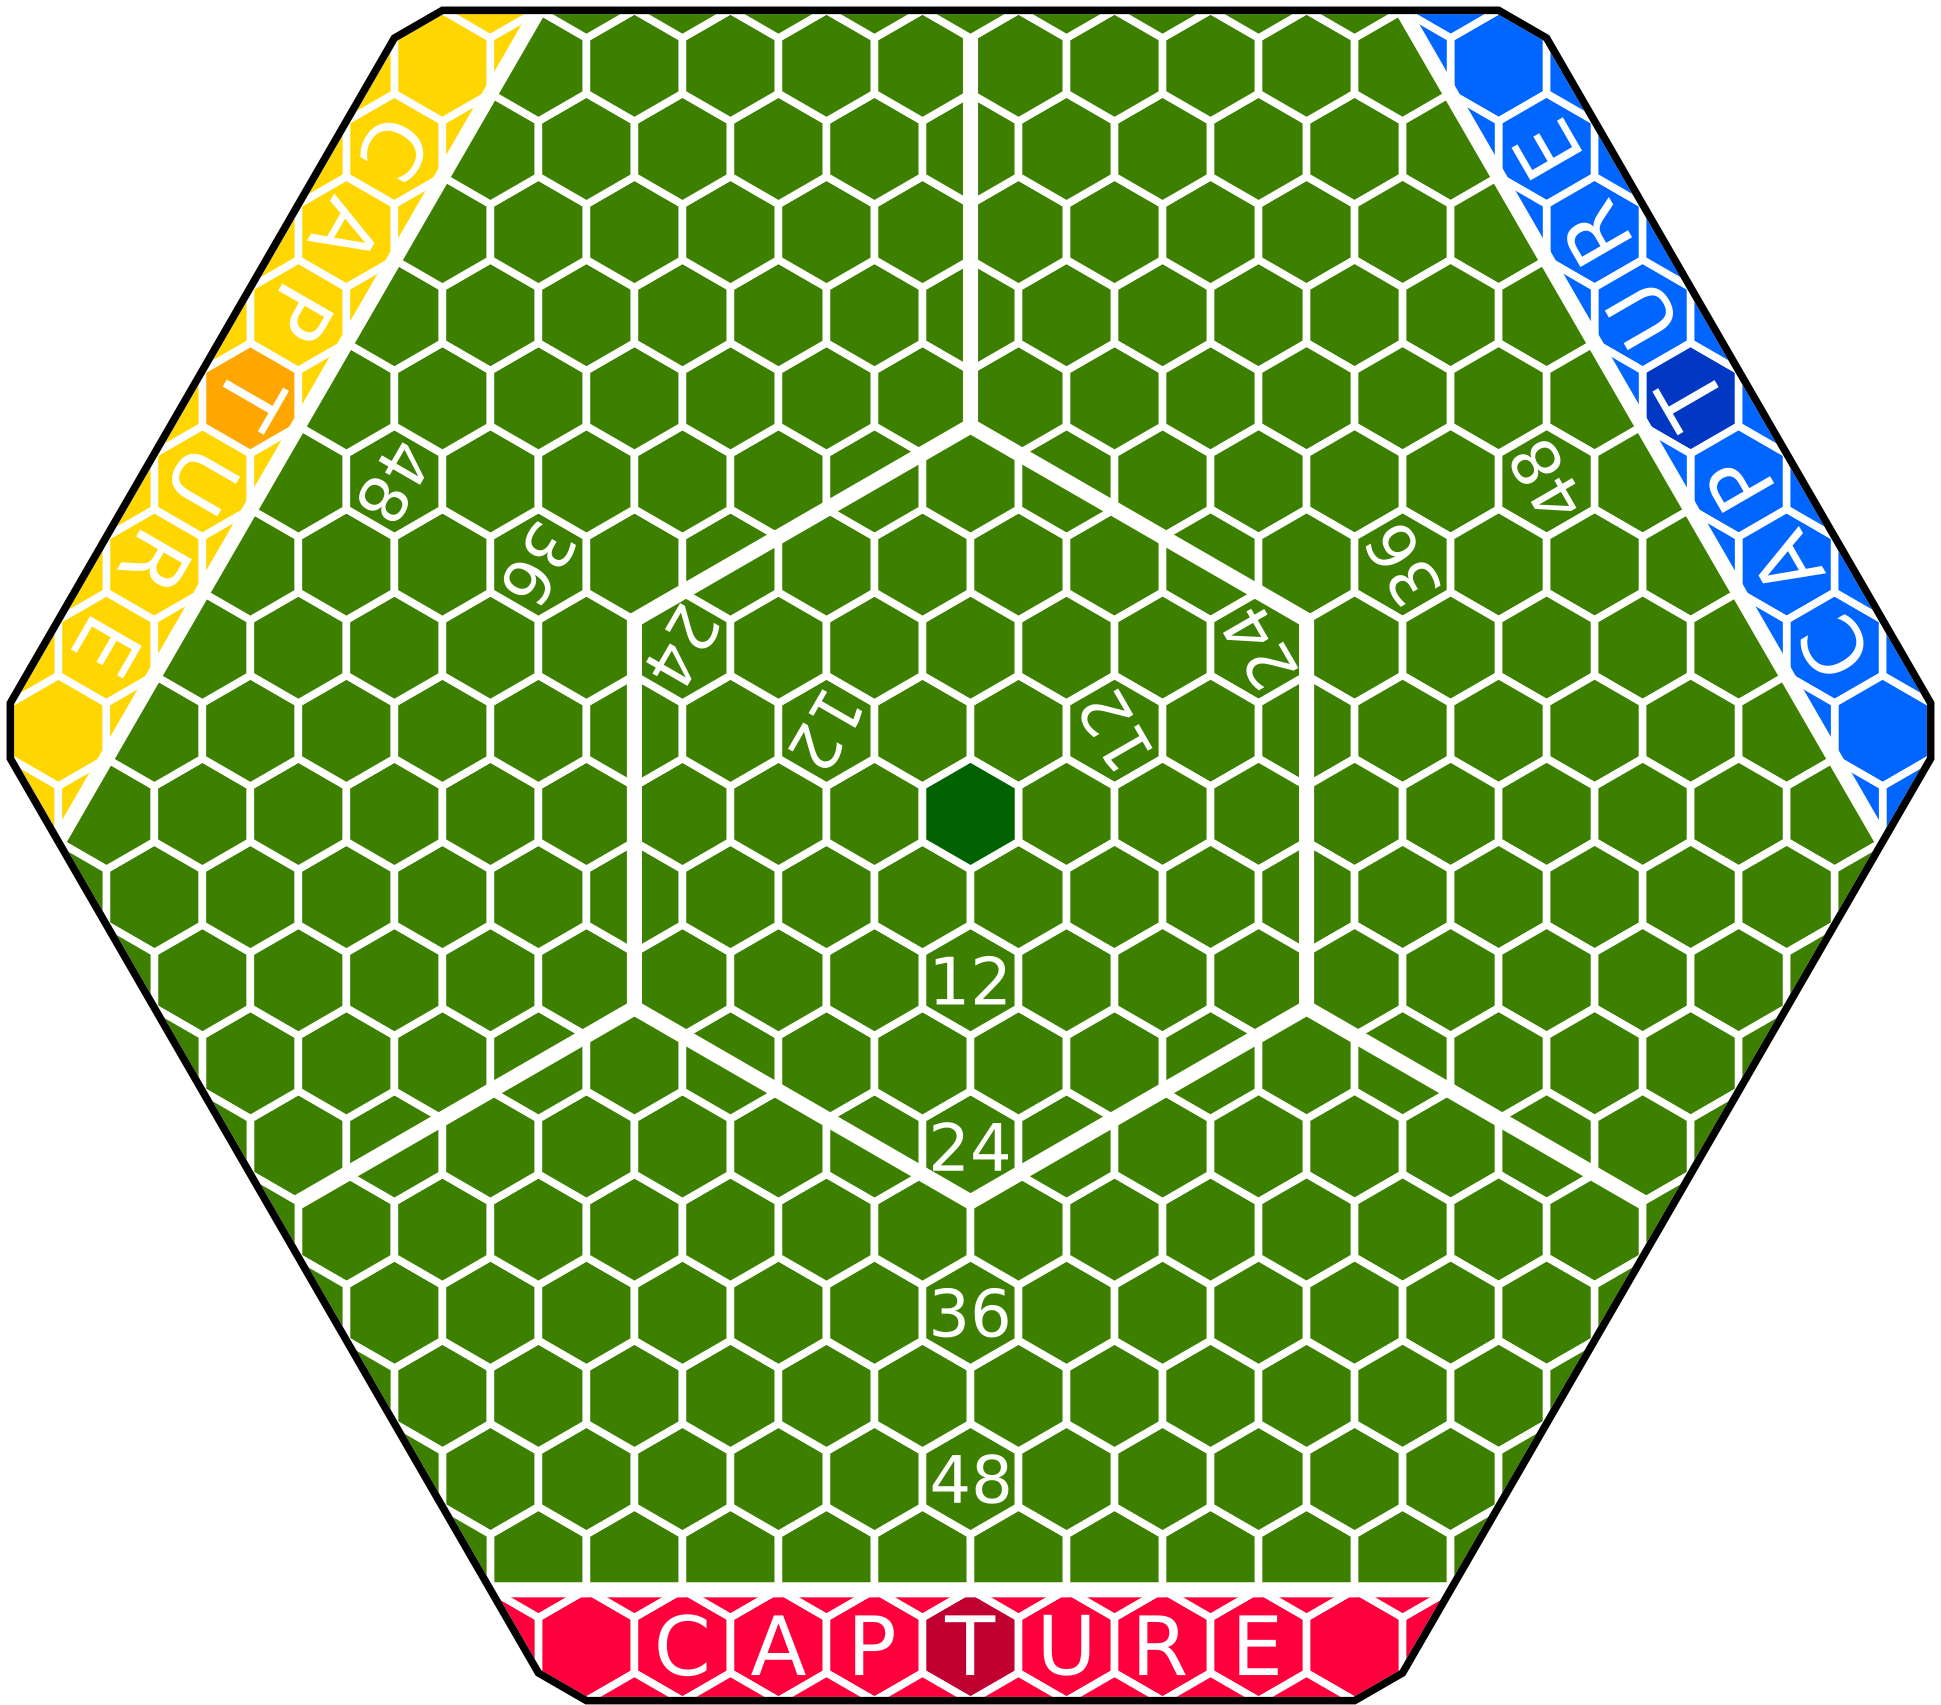
\includegraphics[width=\textwidth]{graphics/board-2}
    \caption{The Playing Field}
    \label{fig:court}
\end{figure}
Depicted on \figref{fig:court} is a mock-up of the playing field.
The three coloured edges are the capture zones.
The darker hexes in each capture zone, is where that team's flag is placed at the start of the game.
The dark hex in the middle is where the ball is placed.
The white lines mark the different teams' starting zones.
The middle zone is a buffer zone where players can’t position their units at the start of the game.

\begin{note}
    From this point onward the people playing the game will be referred to as \textit{coaches} and the figures on the board as \textit{players}.
\end{note}

\section*{Special Thanks}
Special thanks to the lovely individuals who've helped out with the project in one way or another:
\begin{center}
    \begin{tabular}{cccc}
        Epic Panda ApS & Christian J. Martinsen & Marco L. L. Olsen & Barbara Laterman \\ Zach Reedy & Jakob H. Engell\\
    \end{tabular}
\end{center}

\tableofcontents
\mainmatter
\chapter{Terminology}
This chapter simply lists the meaning of various words used throughout this document.

\begin{description}
\item[Character] A character is one of the movable player models.
The characters have different stats as outlined by the Teams chapter.
\item[d6] A six-sided die.
\item[Fate Die] A d6 which has $+$, $-$, and blank on its faces rather than pips/numbers.
\item[Flag] The flag refers to any capturable object within the game, be it the Heavy or the Spear; both are ``flags''.
\item[Player] You, the player.
\item[Skill Roll] Rolling 3d6 against a character's skill level.
Rolling less than or equal to the level is a success, above is a fail.
See Section \ref{skill-rolls} for more details.
\end{description}
\documentclass[a4paper]{book}
\usepackage[utf8]{inputenc}
\usepackage[margin=3cm]{geometry} % For smaller margins
\usepackage{appendix} % For appendix support
\usepackage{tikz, pgfplots} % For the skill outcome graph
    \pgfplotsset{width = \textwidth, compat = newest}
\usepackage{graphicx} % For advanced picture insertion
\usepackage{pdfpages} % For inserting PDFs
\usepackage{multicol} % For supporting multi-columnar tables
\usepackage{tcolorbox} % For coloured info boxes
    \tcbuselibrary{skins}
    \tcbset{colback=brown!10, fonttitle=\scshape}
\usepackage{textcomp} % For the interrobang
\usepackage[sc,sf,bf]{titlesec} % for custom titles
\usepackage{sectsty} % for section styles
\usepackage{fancyhdr} % for "fancy" headers
\usepackage[notmath]{sansmathfonts} % for a sans-serif small-caps font
\usepackage{enumitem} % for finer control over enumerations
 
\usepackage{epsdice}

%%%%%%%%%%%%%%%%%%%%%%%%%%%%%%%%%
%% CHAPTERS & SECTION HEADINGS %%
%%%%%%%%%%%%%%%%%%%%%%%%%%%%%%%%%


% Simplifies chapter titles
% No longer says
% Chapter 2
% Game Creation
% but instead simply
% 2 Game Creation
\titleformat{\chapter}[hang]
{\sffamily\bfseries\scshape\Huge}
{\thechapter\quad}{0pt}{}{}

% Removes unnecessarily large margin above chapter title
\titlespacing*{\chapter}{0pt}{-\topskip}{40pt}

% Set the remaining titles to be sans serif and small caps
\allsectionsfont{\sffamily\scshape}

%%%%%%%%%%%%%%%%%
%% THUMB INDEX %%
%%%%%%%%%%%%%%%%%

\renewcommand{\chaptermark}[1]{\markboth{\textsc{\thechapter\ #1}}{}}

%%%%%%%%%%%%%%%%%%%%%%%
%% CUSTOM TEXT BOXES %%
%%%%%%%%%%%%%%%%%%%%%%%
\newtcolorbox{note}{
    enhanced, % enable advanced settings
    left = 10mm, % pushes text away from the left edge by 10mm
    sharp corners, % disables rounded corners
    rounded corners = southeast, % "round" the bottom right corner
    arc is angular, % make the "round" corner an angle
    arc = 3mm, % controls corner cut
    boxrule=0.6pt, % sets box line thickness
    underlay={%
        \path[fill=tcbcolback!80!black] ([yshift=3mm]interior.south east)--++(-0.4,-0.1)--++(0.1,-0.2); % triangle
        \path[draw=tcbcolframe,shorten <=-0.05mm,shorten >=-0.05mm] ([yshift=3mm]interior.south east)--++(-0.4,-0.1)--++(0.1,-0.2); % triangle edge
        \path[fill=gray!50!black,draw=none] (interior.south west) rectangle node[brown!10]{\Huge\bfseries \textinterrobang} ([xshift=8mm]interior.north west);
    },
    drop fuzzy shadow % adds drop shadow
}

\newtcolorbox{example}{
    enhanced,
    title = Example,
    before upper={\parindent15pt\noindent} % add paragraph indentation
}

\begin{document}

\begin{titlepage}
\begin{center}
    \huge{\textbf{FLAG-BALL}}\\
    \LARGE{
        $\alpha1.0.0$\\
        By Alex Laterman \& Niko Lepka
    }\\
    \Large{\today}
\end{center}
\end{titlepage}
\thispagestyle{empty} % removes page number from front page
\frontmatter % adds Roman numerals to the preface chapter

\section*{Premise}
Flag-Ball is a rugby/capture-the-flag hybrid tabletop game for three players.
Each player has a flag to protect, and a team of characters.
The game is played on a hex-grid, with three of the sides acting as each team's capture zone.
\begin{figure}
    \centering
    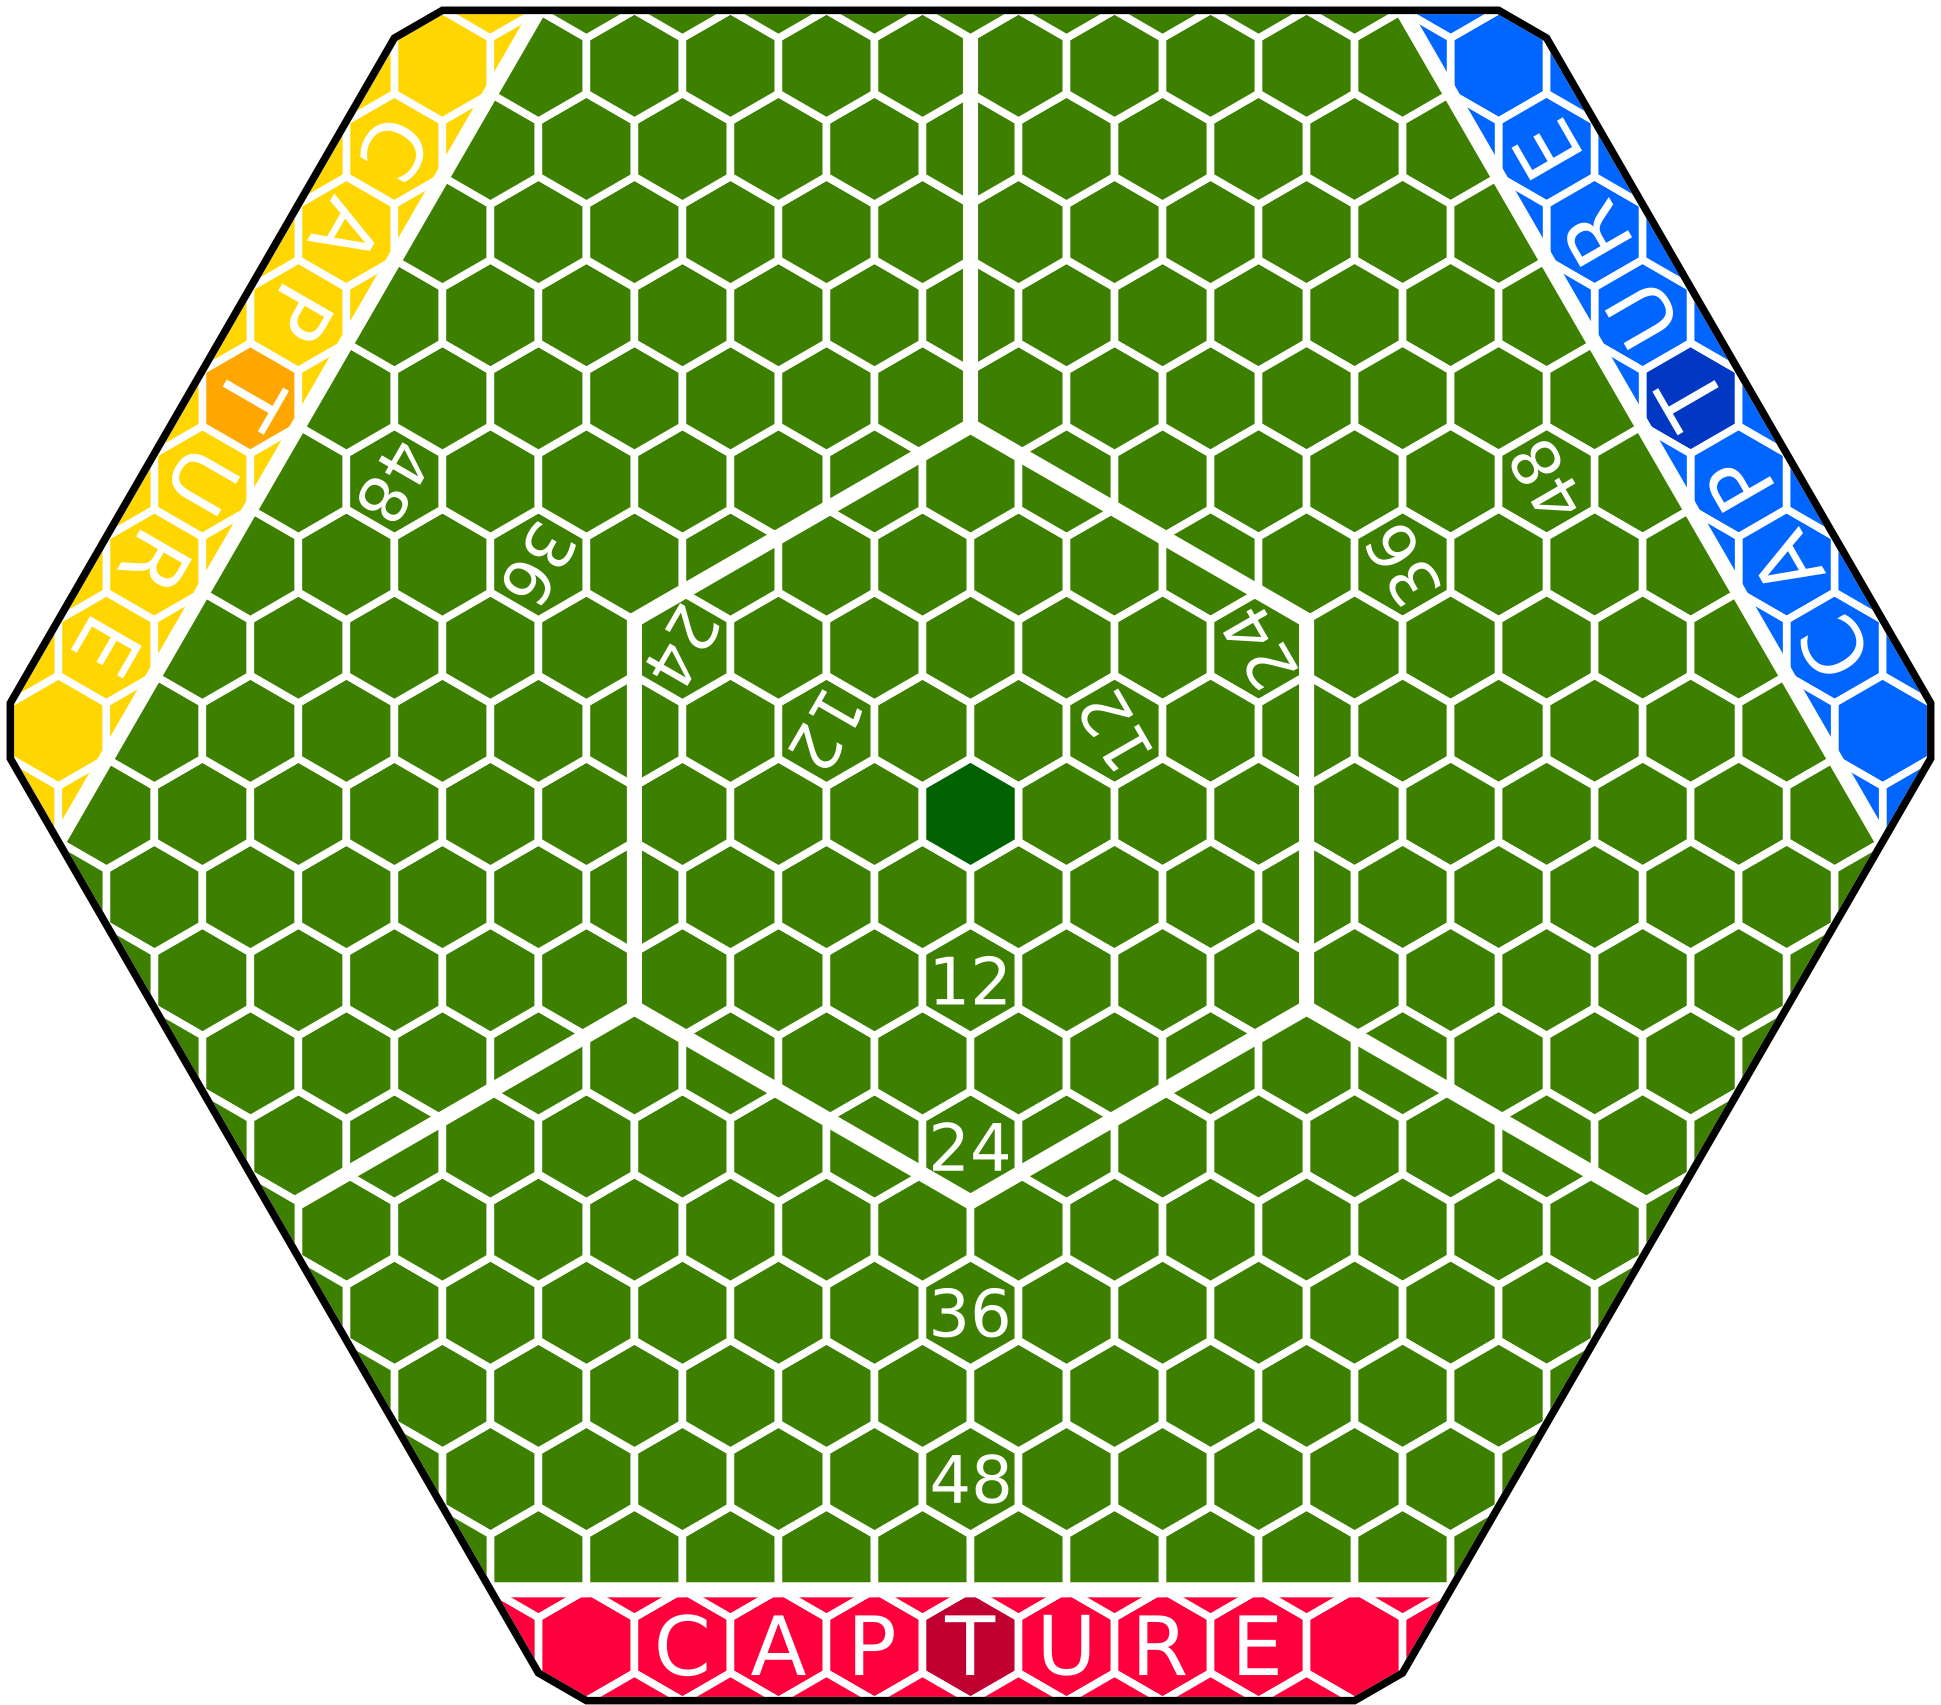
\includegraphics[width=\textwidth]{graphics/board-2}
    \caption{The Playing Field}
    \label{fig:court}
\end{figure}
Depicted on Figure \ref{fig:court} is a mock-up of the playing field.
The three coloured edges are the capture zones.
The darker hexes in each capture zone, is where that team's flag is placed at the start of the game.
The dark hex in the middle is where \textit{The Heavy} is placed.
The white lines mark the different teams' starting zones.
The middle zone is a buffer zone where players can’t position their units at the start of the game.

\section*{Special Thanks}
Special thanks to the lovely individuals who've helped out with the project in one way or another:
\begin{center}
    \begin{tabular}{cccc}
        Epic Panda ApS & Christian J. Martinsen & Marco L. L. Olsen\\
    \end{tabular}
\end{center}

\tableofcontents
\mainmatter
\documentclass[a4paper]{book}
\usepackage[utf8]{inputenc}
\usepackage[margin=3cm]{geometry} % For smaller margins
\usepackage{appendix} % For appendix support
\usepackage{tikz, pgfplots} % For the skill outcome graph
    \pgfplotsset{width = \textwidth, compat = newest}
\usepackage{graphicx} % For advanced picture insertion
\usepackage{pdfpages} % For inserting PDFs
\usepackage{multicol} % For supporting multi-columnar tables
\usepackage{tcolorbox} % For coloured info boxes
    \tcbuselibrary{skins}
    \tcbset{colback=brown!10, fonttitle=\scshape}
\usepackage{textcomp} % For the interrobang
\usepackage[sc,sf,bf]{titlesec} % for custom titles
\usepackage{sectsty} % for section styles
\usepackage{fancyhdr} % for "fancy" headers
\usepackage[notmath]{sansmathfonts} % for a sans-serif small-caps font
\usepackage{enumitem} % for finer control over enumerations
 
\usepackage{epsdice}

%%%%%%%%%%%%%%%%%%%%%%%%%%%%%%%%%
%% CHAPTERS & SECTION HEADINGS %%
%%%%%%%%%%%%%%%%%%%%%%%%%%%%%%%%%


% Simplifies chapter titles
% No longer says
% Chapter 2
% Game Creation
% but instead simply
% 2 Game Creation
\titleformat{\chapter}[hang]
{\sffamily\bfseries\scshape\Huge}
{\thechapter\quad}{0pt}{}{}

% Removes unnecessarily large margin above chapter title
\titlespacing*{\chapter}{0pt}{-\topskip}{40pt}

% Set the remaining titles to be sans serif and small caps
\allsectionsfont{\sffamily\scshape}

%%%%%%%%%%%%%%%%%
%% THUMB INDEX %%
%%%%%%%%%%%%%%%%%

\renewcommand{\chaptermark}[1]{\markboth{\textsc{\thechapter\ #1}}{}}

%%%%%%%%%%%%%%%%%%%%%%%
%% CUSTOM TEXT BOXES %%
%%%%%%%%%%%%%%%%%%%%%%%
\newtcolorbox{note}{
    enhanced, % enable advanced settings
    left = 10mm, % pushes text away from the left edge by 10mm
    sharp corners, % disables rounded corners
    rounded corners = southeast, % "round" the bottom right corner
    arc is angular, % make the "round" corner an angle
    arc = 3mm, % controls corner cut
    boxrule=0.6pt, % sets box line thickness
    underlay={%
        \path[fill=tcbcolback!80!black] ([yshift=3mm]interior.south east)--++(-0.4,-0.1)--++(0.1,-0.2); % triangle
        \path[draw=tcbcolframe,shorten <=-0.05mm,shorten >=-0.05mm] ([yshift=3mm]interior.south east)--++(-0.4,-0.1)--++(0.1,-0.2); % triangle edge
        \path[fill=gray!50!black,draw=none] (interior.south west) rectangle node[brown!10]{\Huge\bfseries \textinterrobang} ([xshift=8mm]interior.north west);
    },
    drop fuzzy shadow % adds drop shadow
}

\newtcolorbox{example}{
    enhanced,
    title = Example,
    before upper={\parindent15pt\noindent} % add paragraph indentation
}

\begin{document}

\begin{titlepage}
\begin{center}
    \huge{\textbf{FLAG-BALL}}\\
    \LARGE{
        $\alpha1.0.0$\\
        By Alex Laterman \& Niko Lepka
    }\\
    \Large{\today}
\end{center}
\end{titlepage}
\thispagestyle{empty} % removes page number from front page
\frontmatter % adds Roman numerals to the preface chapter

\section*{Premise}
Flag-Ball is a rugby/capture-the-flag hybrid tabletop game for three players.
Each player has a flag to protect, and a team of characters.
The game is played on a hex-grid, with three of the sides acting as each team's capture zone.
\begin{figure}
    \centering
    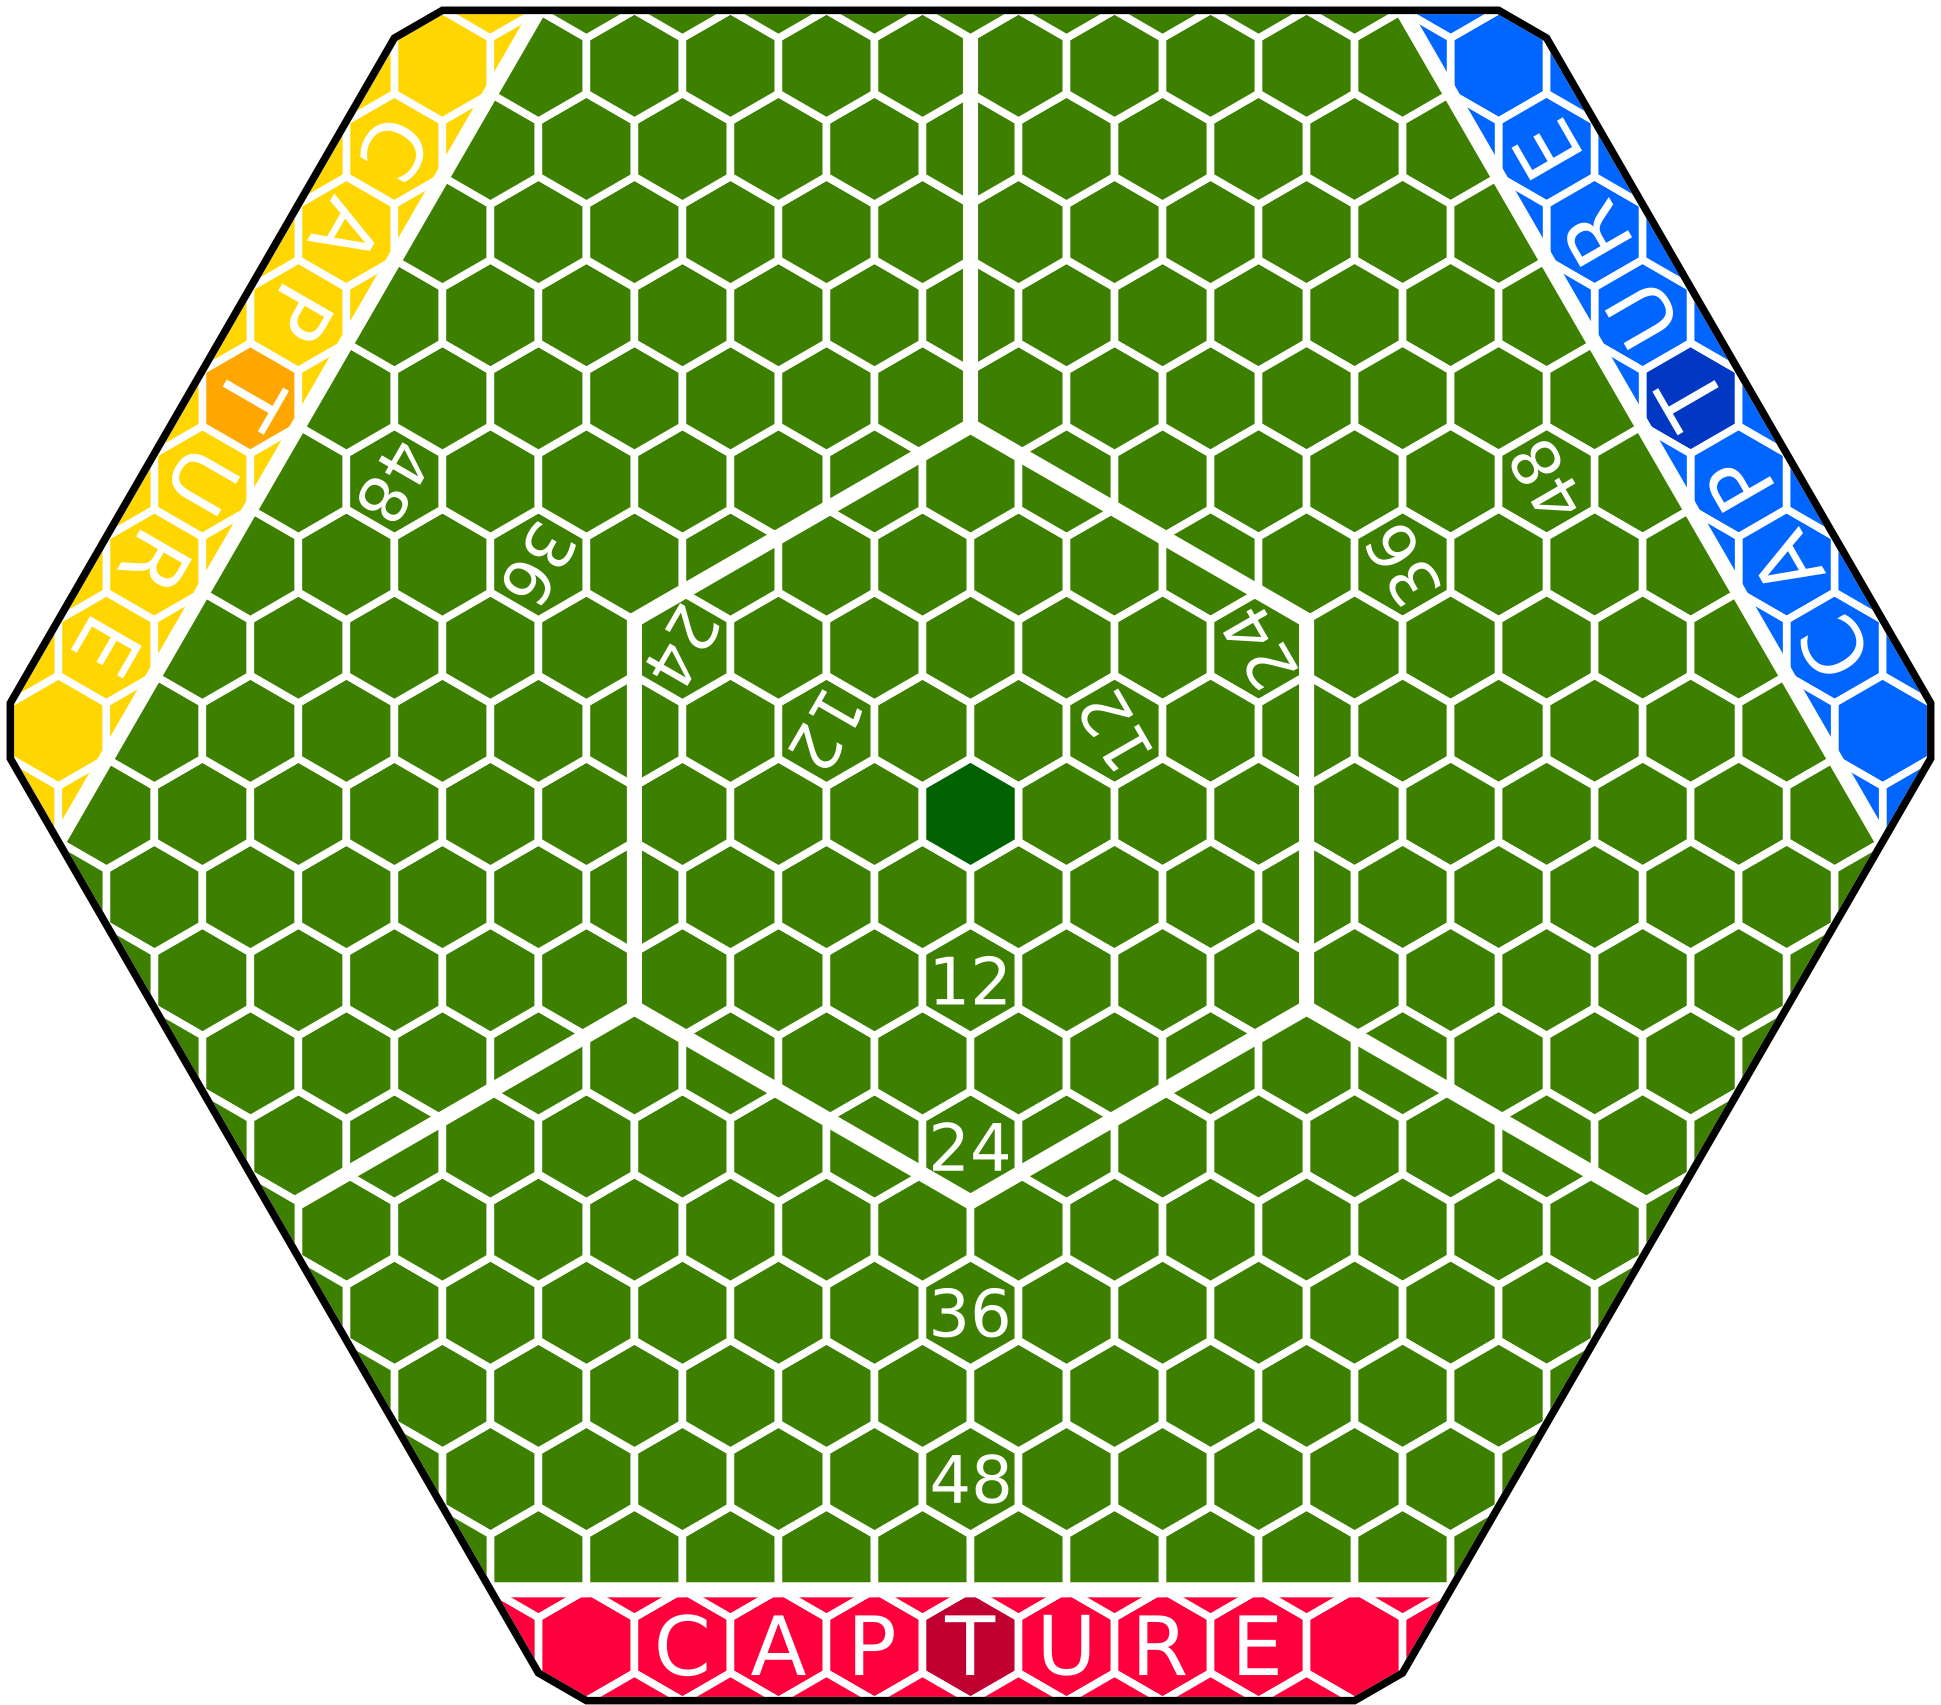
\includegraphics[width=\textwidth]{graphics/board-2}
    \caption{The Playing Field}
    \label{fig:court}
\end{figure}
Depicted on Figure \ref{fig:court} is a mock-up of the playing field.
The three coloured edges are the capture zones.
The darker hexes in each capture zone, is where that team's flag is placed at the start of the game.
The dark hex in the middle is where \textit{The Heavy} is placed.
The white lines mark the different teams' starting zones.
The middle zone is a buffer zone where players can’t position their units at the start of the game.

\section*{Special Thanks}
Special thanks to the lovely individuals who've helped out with the project in one way or another:
\begin{center}
    \begin{tabular}{cccc}
        Epic Panda ApS & Christian J. Martinsen & Marco L. L. Olsen\\
    \end{tabular}
\end{center}

\tableofcontents
\mainmatter
\documentclass[a4paper]{book}
\input{preamble.tex}

\begin{document}

\begin{titlepage}
\begin{center}
    \huge{\textbf{FLAG-BALL}}\\
    \LARGE{
        $\alpha1.0.0$\\
        By Alex Laterman \& Niko Lepka
    }\\
    \Large{\today}
\end{center}
\end{titlepage}
\thispagestyle{empty} % removes page number from front page
\frontmatter % adds Roman numerals to the preface chapter

\section*{Premise}
Flag-Ball is a rugby/capture-the-flag hybrid tabletop game for three players.
Each player has a flag to protect, and a team of characters.
The game is played on a hex-grid, with three of the sides acting as each team's capture zone.
\begin{figure}
    \centering
    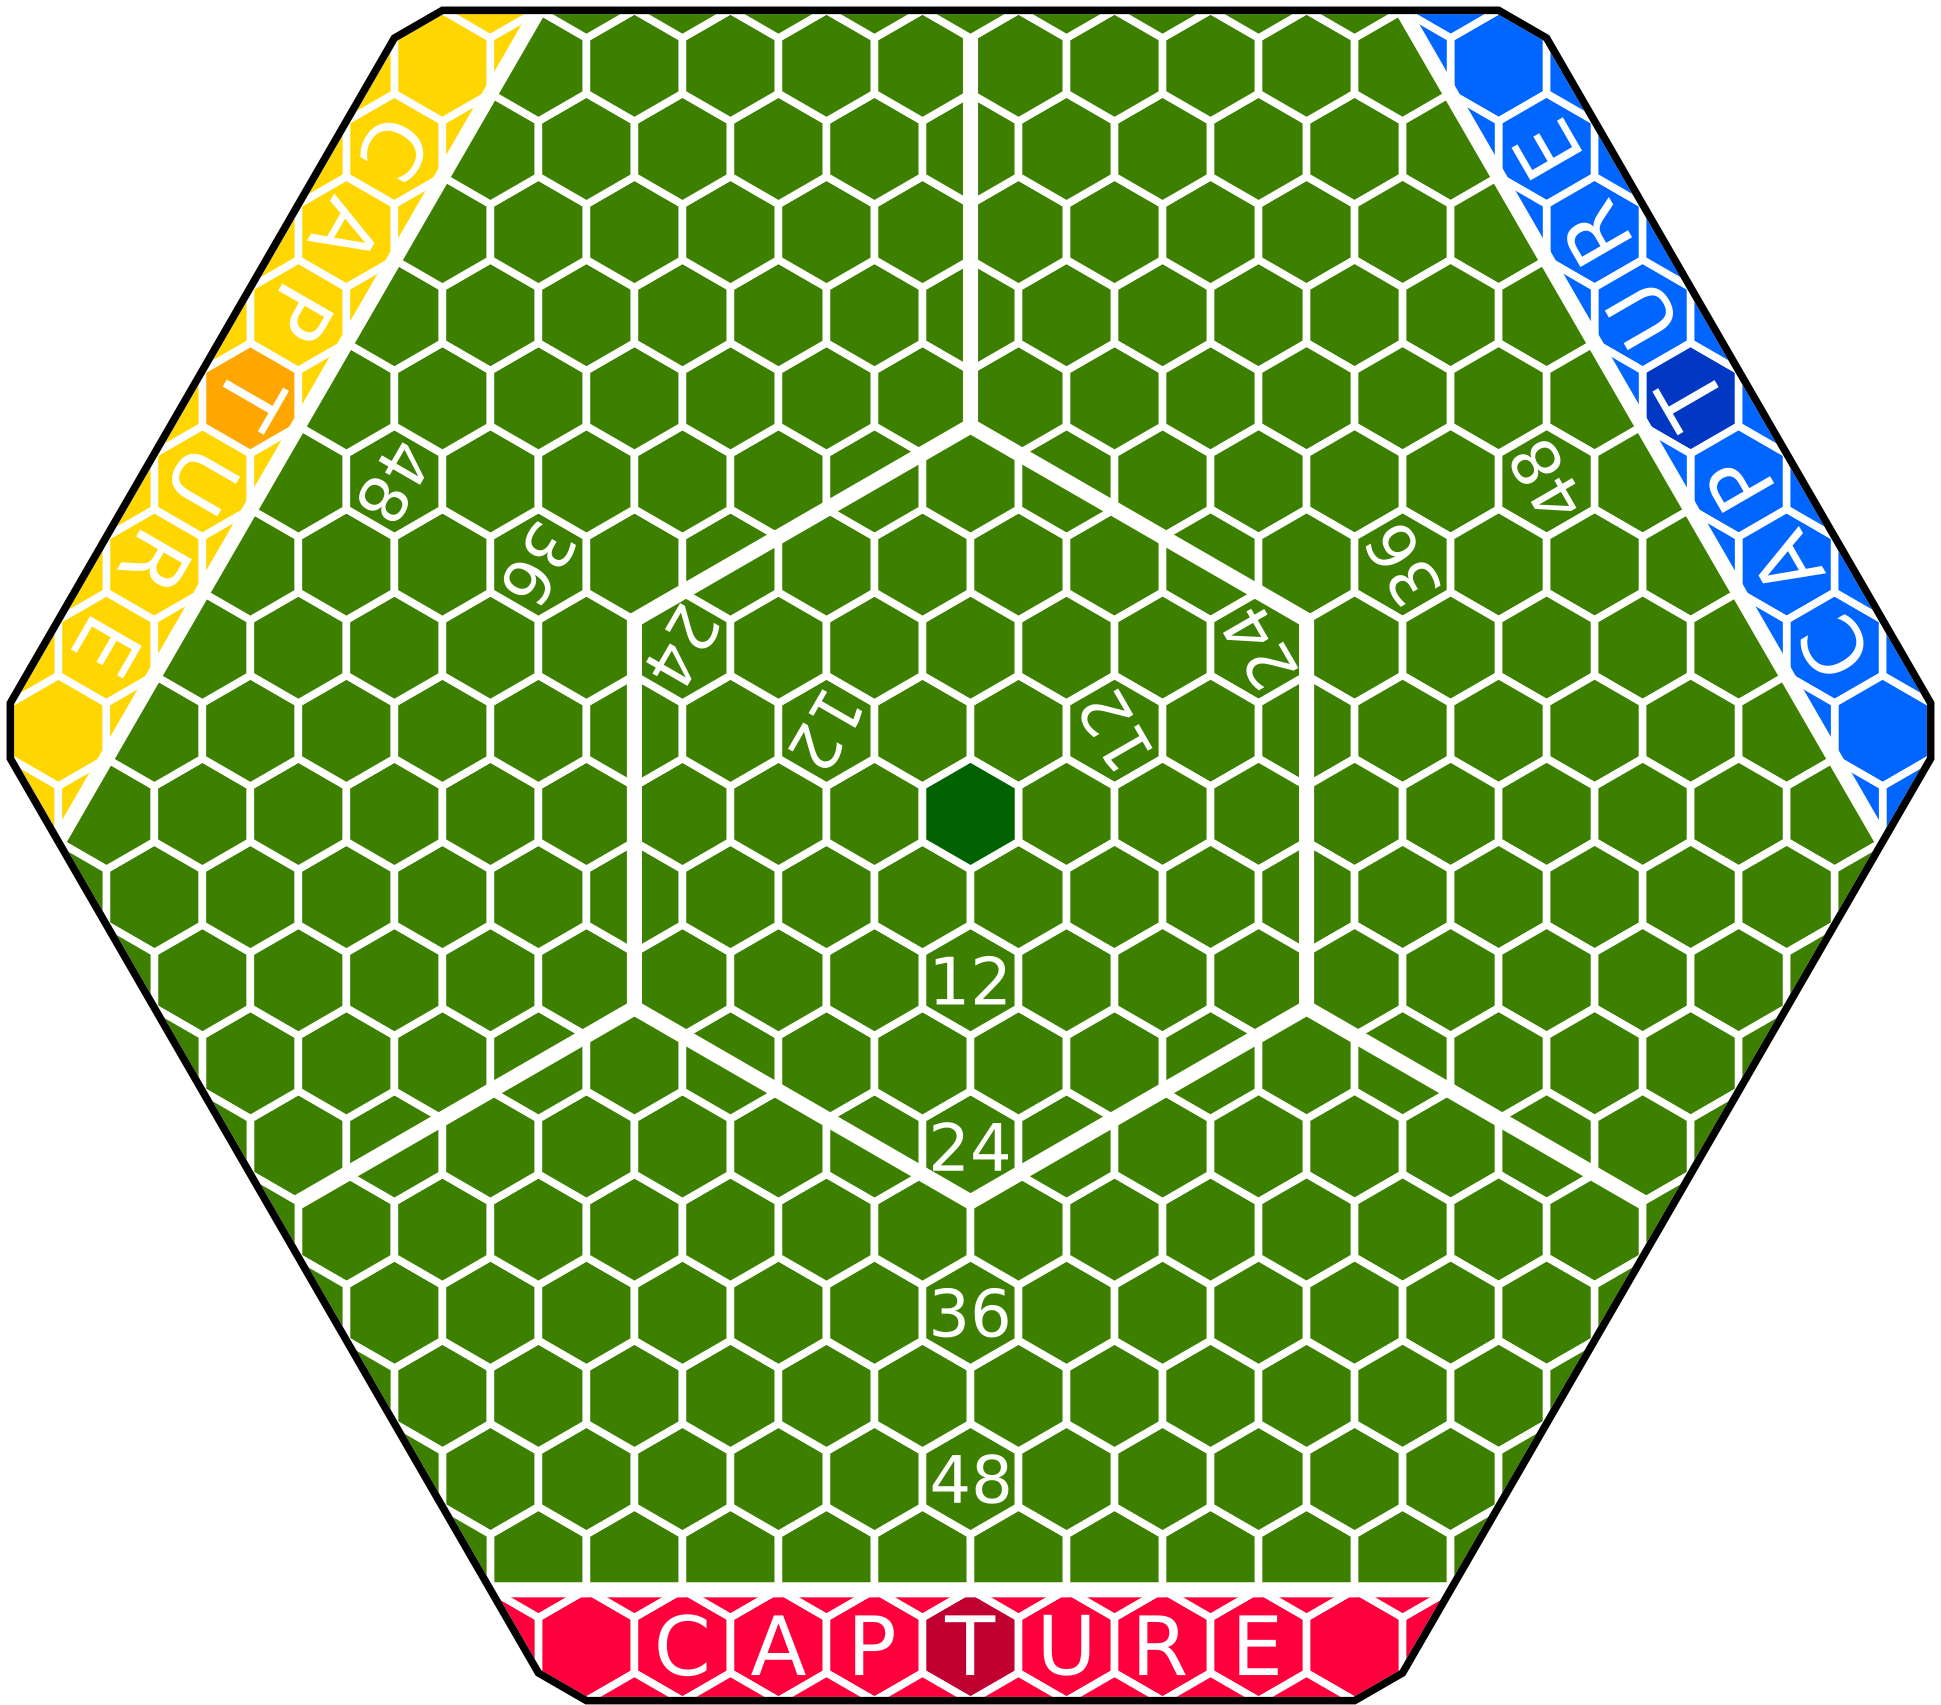
\includegraphics[width=\textwidth]{graphics/board-2}
    \caption{The Playing Field}
    \label{fig:court}
\end{figure}
Depicted on Figure \ref{fig:court} is a mock-up of the playing field.
The three coloured edges are the capture zones.
The darker hexes in each capture zone, is where that team's flag is placed at the start of the game.
The dark hex in the middle is where \textit{The Heavy} is placed.
The white lines mark the different teams' starting zones.
The middle zone is a buffer zone where players can’t position their units at the start of the game.

\section*{Special Thanks}
Special thanks to the lovely individuals who've helped out with the project in one way or another:
\begin{center}
    \begin{tabular}{cccc}
        Epic Panda ApS & Christian J. Martinsen & Marco L. L. Olsen\\
    \end{tabular}
\end{center}

\tableofcontents
\mainmatter
\input{chapters/the-game/main.tex}
\input{chapters/teams.tex}
\input{chapters/terminology.tex}
\input{chapters/outcome-table.tex}
\end{document}

\chapter{Teams}
This chapter includes some stats of some premade team compositions and their associated players.
\section{Team Alpha}
The Play-test team.
It consists of
\begin{itemize}
    \item 1 Runner
    \item 2 Pitchers
    \item 2 Bruisers
    \item 2 Defenders
\end{itemize}

\subsection{Runner}
\begin{center}
\begin{tabular}{r|p{5cm}}
    \textbf{Agility} & 12 \\
    \textbf{Dexterity} & 10 \\
    \textbf{Strength} & 10 \\ \hline
    \textbf{Move} & 6 ($Agi/2=6$)\\
    \textbf{Throw} & 5 ($Dex/2=5$) \\ \hline
    \textbf{Abilities} & \textbf{See Ya!} (Cost: 2) -- Move 3 additional hexes.
\end{tabular}
\end{center}

\subsection{Pitcher}
\begin{center}
\begin{tabular}{r|p{5cm}}
    \textbf{Agility} & 10 \\
    \textbf{Dexterity} & 12 \\
    \textbf{Strength} & 10 \\ \hline
    \textbf{Move} & 5 ($Agi/2=5$)\\
    \textbf{Throw} & 6 ($Dex/2=6$) \\ \hline
    \textbf{Abilities} & \textbf{Yoink} (Cost: 1) -- Move immediately after picking up a flag, if any movement points remain.
\end{tabular}
\end{center}

\subsection{Bruiser}
\begin{center}
\begin{tabular}{r|p{5cm}}
    \textbf{Agility} & 10 \\
    \textbf{Dexterity} & 10 \\
    \textbf{Strength} & 12 \\ \hline
    \textbf{Move} & 5 ($Agi/2=5$)\\
    \textbf{Throw} & 5 ($Dex/2=5$) \\ \hline
    \textbf{Abilities} & \textbf{Smash!} (Cost: 3) -- +1 to attack.
    Attack all opponents within 1 hex of Bruiser.
\end{tabular}
\end{center}

\subsection{Defender}
\begin{center}
\begin{tabular}{r|p{5cm}}
    \textbf{Agility} & 10 \\
    \textbf{Dexterity} & 10 \\
    \textbf{Strength} & 10 \\ \hline
    \textbf{Move} & 5 ($Agi/2=5$)\\
    \textbf{Throw} & 5 ($Dex/2=5$) \\ \hline
    \textbf{Abilities} & \textbf{Blockade} (Cost: 0) -- Opponents have $-2$ to any skill roll made against the defender.
\end{tabular}
\end{center}

The Defender's skill may be a bit confusing to some, so here's a more in-depth explanation of what this means: If your Defender is attacked by an opponent's Pitcher, instead of rolling under 10 to succeed the attack, they have to roll under 8 ($Str-2=8$) to succeed.
Similarly, if a Runner wants to exit the Defender's tackle zone, they have to roll under 10 ($Agi-2=10$) to succeed.

This gives the Defender tremendous \textit{pinning power}, in that they can effectively deny opponents passage.
\chapter{Terminology}
This chapter simply lists the meaning of various words used throughout this document.

\begin{description}
\item[Character] A character is one of the movable player models.
The characters have different stats as outlined by the Teams chapter.
\item[d6] A six-sided die.
\item[Fate Die] A d6 which has $+$, $-$, and blank on its faces rather than pips/numbers.
\item[Flag] The flag refers to any capturable object within the game, be it the Heavy or the Spear; both are ``flags''.
\item[Player] You, the player.
\item[Skill Roll] Rolling 3d6 against a character's skill level.
Rolling less than or equal to the level is a success, above is a fail.
See Section \ref{skill-rolls} for more details.
\end{description}
\chapter{Charts \& Tables}
\section{Skill Roll Outcome Graph}
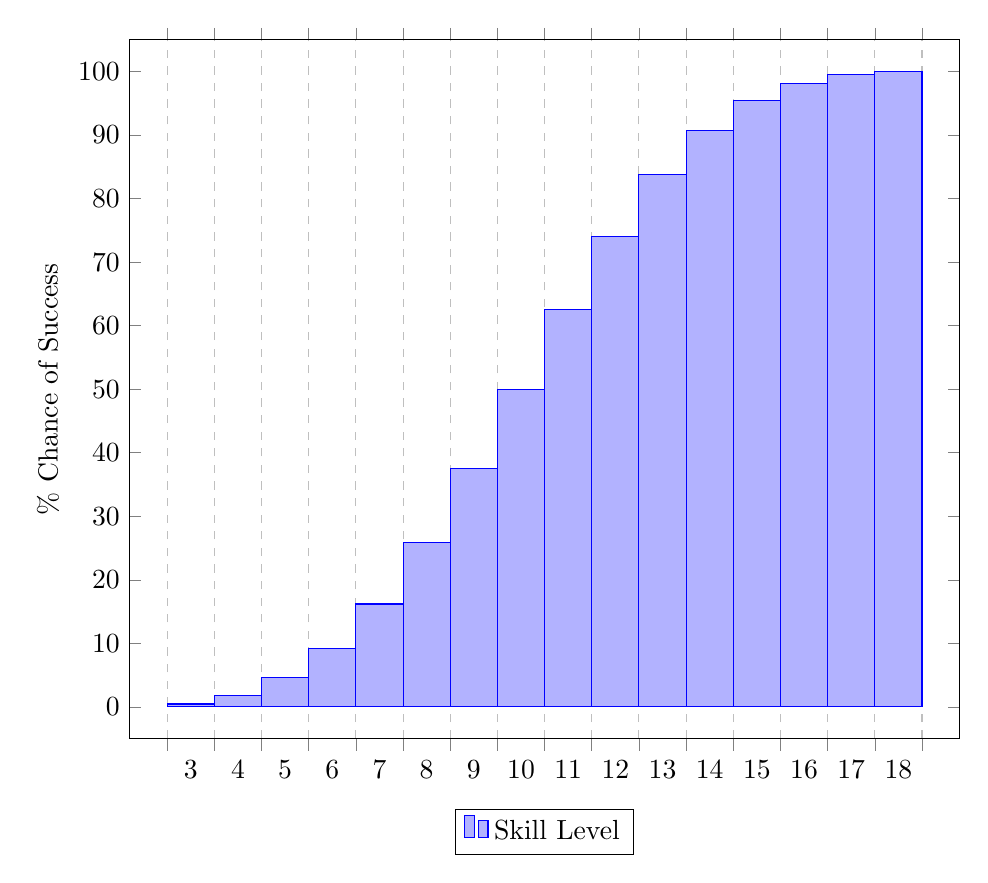
\begin{tikzpicture}
\begin{axis}[
	x tick label style={/pgf/number format/1000 sep=},
	ylabel=\% Chance of Success,
	enlargelimits=0.05,
	ytick = {0, 10, 20, 30, 40, 50, 60, 70, 80, 90, 100},
	legend style = {
	    at={(0.5,-0.1)},
	    grid style = dashed,
	    anchor=north,legend columns=-1
	},
	ybar interval = 1,
]
\addplot 
	coordinates {
	    (3, 0.46) 
	    (4, 1.85)
		(5, 4.63) 
		(6, 9.26) 
		(7, 16.20) 
		(8, 25.93) 
		(9, 37.50) 
		(10, 50.00) 
		(11, 62.50) 
		(12, 74.07)
		(13, 83.80)
		(14, 90.74)
		(15, 95.37)
		(16, 98.15)
		(17, 99.54)
		(18, 100.00)
		(19, 0)
	};
\legend{Skill Level}
\end{axis}
\end{tikzpicture}\\
The graph above shows the probability of succeeding a skill roll.
If your character has an effective skill of 10, they have a 50\% chance of succeeding that roll.
If they have a skill of 12, the chance of success goes up to 74\%.
\end{document}

\chapter{Teams}
This chapter includes some stats of some premade team compositions and their associated players.
\section{Team Alpha}
The Play-test team.
It consists of
\begin{itemize}
    \item 1 Runner
    \item 2 Pitchers
    \item 2 Bruisers
    \item 2 Defenders
\end{itemize}

\subsection{Runner}
\begin{center}
\begin{tabular}{r|p{5cm}}
    \textbf{Agility} & 12 \\
    \textbf{Dexterity} & 10 \\
    \textbf{Strength} & 10 \\ \hline
    \textbf{Move} & 6 ($Agi/2=6$)\\
    \textbf{Throw} & 5 ($Dex/2=5$) \\ \hline
    \textbf{Abilities} & \textbf{See Ya!} (Cost: 2) -- Move 3 additional hexes.
\end{tabular}
\end{center}

\subsection{Pitcher}
\begin{center}
\begin{tabular}{r|p{5cm}}
    \textbf{Agility} & 10 \\
    \textbf{Dexterity} & 12 \\
    \textbf{Strength} & 10 \\ \hline
    \textbf{Move} & 5 ($Agi/2=5$)\\
    \textbf{Throw} & 6 ($Dex/2=6$) \\ \hline
    \textbf{Abilities} & \textbf{Yoink} (Cost: 1) -- Move immediately after picking up a flag, if any movement points remain.
\end{tabular}
\end{center}

\subsection{Bruiser}
\begin{center}
\begin{tabular}{r|p{5cm}}
    \textbf{Agility} & 10 \\
    \textbf{Dexterity} & 10 \\
    \textbf{Strength} & 12 \\ \hline
    \textbf{Move} & 5 ($Agi/2=5$)\\
    \textbf{Throw} & 5 ($Dex/2=5$) \\ \hline
    \textbf{Abilities} & \textbf{Smash!} (Cost: 3) -- +1 to attack.
    Attack all opponents within 1 hex of Bruiser.
\end{tabular}
\end{center}

\subsection{Defender}
\begin{center}
\begin{tabular}{r|p{5cm}}
    \textbf{Agility} & 10 \\
    \textbf{Dexterity} & 10 \\
    \textbf{Strength} & 10 \\ \hline
    \textbf{Move} & 5 ($Agi/2=5$)\\
    \textbf{Throw} & 5 ($Dex/2=5$) \\ \hline
    \textbf{Abilities} & \textbf{Blockade} (Cost: 0) -- Opponents have $-2$ to any skill roll made against the defender.
\end{tabular}
\end{center}

The Defender's skill may be a bit confusing to some, so here's a more in-depth explanation of what this means: If your Defender is attacked by an opponent's Pitcher, instead of rolling under 10 to succeed the attack, they have to roll under 8 ($Str-2=8$) to succeed.
Similarly, if a Runner wants to exit the Defender's tackle zone, they have to roll under 10 ($Agi-2=10$) to succeed.

This gives the Defender tremendous \textit{pinning power}, in that they can effectively deny opponents passage.
\chapter{Terminology}
This chapter simply lists the meaning of various words used throughout this document.

\begin{description}
\item[Character] A character is one of the movable player models.
The characters have different stats as outlined by the Teams chapter.
\item[d6] A six-sided die.
\item[Fate Die] A d6 which has $+$, $-$, and blank on its faces rather than pips/numbers.
\item[Flag] The flag refers to any capturable object within the game, be it the Heavy or the Spear; both are ``flags''.
\item[Player] You, the player.
\item[Skill Roll] Rolling 3d6 against a character's skill level.
Rolling less than or equal to the level is a success, above is a fail.
See Section \ref{skill-rolls} for more details.
\end{description}
\chapter{Charts \& Tables}
\section{Skill Roll Outcome Graph}
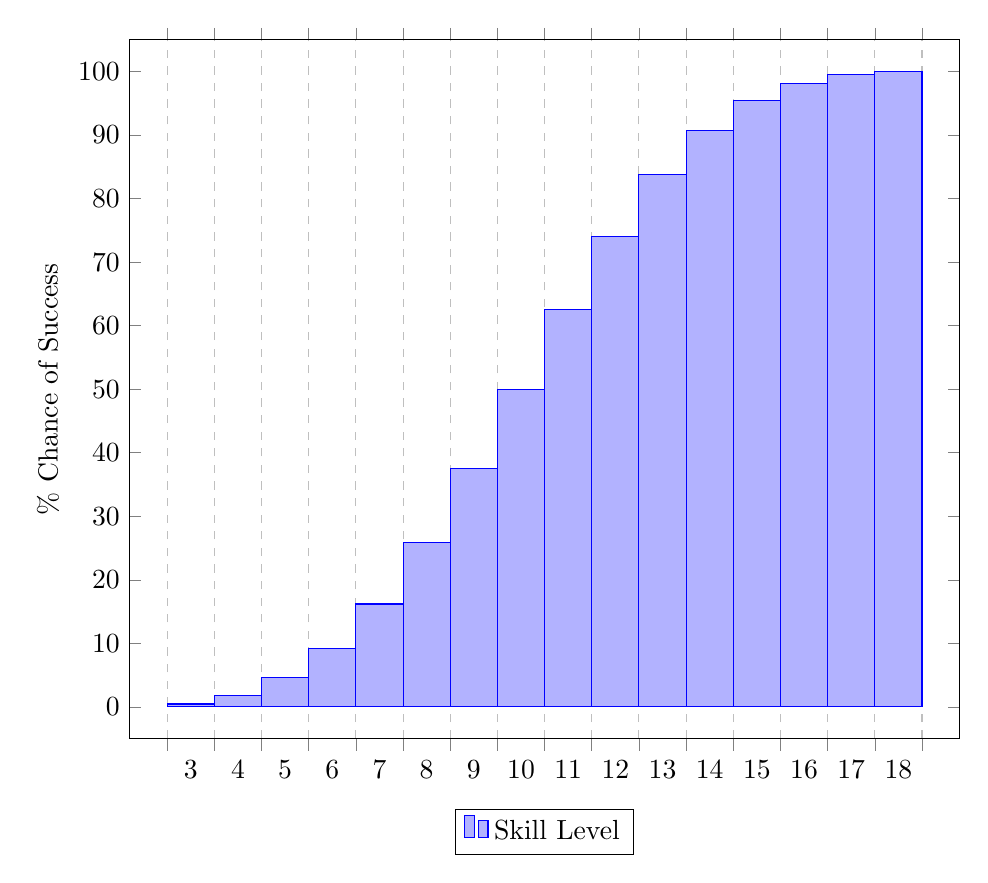
\begin{tikzpicture}
\begin{axis}[
	x tick label style={/pgf/number format/1000 sep=},
	ylabel=\% Chance of Success,
	enlargelimits=0.05,
	ytick = {0, 10, 20, 30, 40, 50, 60, 70, 80, 90, 100},
	legend style = {
	    at={(0.5,-0.1)},
	    grid style = dashed,
	    anchor=north,legend columns=-1
	},
	ybar interval = 1,
]
\addplot 
	coordinates {
	    (3, 0.46) 
	    (4, 1.85)
		(5, 4.63) 
		(6, 9.26) 
		(7, 16.20) 
		(8, 25.93) 
		(9, 37.50) 
		(10, 50.00) 
		(11, 62.50) 
		(12, 74.07)
		(13, 83.80)
		(14, 90.74)
		(15, 95.37)
		(16, 98.15)
		(17, 99.54)
		(18, 100.00)
		(19, 0)
	};
\legend{Skill Level}
\end{axis}
\end{tikzpicture}\\
The graph above shows the probability of succeeding a skill roll.
If your character has an effective skill of 10, they have a 50\% chance of succeeding that roll.
If they have a skill of 12, the chance of success goes up to 74\%.
\end{document}

\appendix
%\chapter{Teams}
This chapter includes some stats of some premade team compositions and their associated players.
\section{Team Alpha}
The Play-test team. It consists of
\begin{itemize}
    \item 1 Runner
    \item 2 Pitchers
    \item 2 Bruisers
    \item 2 Defenders
\end{itemize}

\subsection{Runner}
\begin{tabular}{r|l}
    \textbf{Agility} & 12 \\
    \textbf{Dexterity} & 10 \\
    \textbf{Strength} & 10 \\ \hline
    \textbf{Move} & 6 ($Agi/2=6$)\\
    \textbf{Throw} & 5 ($Dex/2=5$) \\ \hline
    \textbf{Abilities} & None.
\end{tabular}

\subsection{Pitcher}
\begin{tabular}{r|l}
    \textbf{Agility} & 10 \\
    \textbf{Dexterity} & 12 \\
    \textbf{Strength} & 10 \\ \hline
    \textbf{Move} & 5 ($Agi/2=5$)\\
    \textbf{Throw} & 6 ($Dex/2=6$) \\ \hline
    \textbf{Abilities} & \textbf{Yoink} Can move immediately after picking up a flag, if any movement points remain.
\end{tabular}

\subsection{Bruiser}
\begin{tabular}{r|l}
    \textbf{Agility} & 10 \\
    \textbf{Dexterity} & 10 \\
    \textbf{Strength} & 12 \\ \hline
    \textbf{Move} & 5 ($Agi/2=5$)\\
    \textbf{Throw} & 5 ($Dex/2=5$) \\ \hline
    \textbf{Abilities} & None.
\end{tabular}

\subsection{Defender}
\begin{tabular}{r|l}
    \textbf{Agility} & 10 \\
    \textbf{Dexterity} & 10 \\
    \textbf{Strength} & 10 \\ \hline
    \textbf{Move} & 5 ($Agi/2=5$)\\
    \textbf{Throw} & 5 ($Dex/2=5$) \\ \hline
    \textbf{Abilities} & \textbf{Blockade} Opponents have $-2$ to any skill roll made against the defender.
\end{tabular}

The Defender's skill may be a bit confusing to some, so here's a more in-depth explanation of what this means: If your Defender is attacked by an opponent's Pitcher, instead of rolling under 10 to succeed the attack, they have to roll under 8 ($Str-2=8$) to succeed. Similarly, if a Runner wants to exit the Defender's tackle zone, they have to roll under 10 ($Agi-2=10$) to succeed.

This gives the Defender tremendous \textit{pinning power}, in that they can effectively deny opponents passage.
%\chapter{Charts \& Tables}
\section{Skill Roll Outcome Graph}
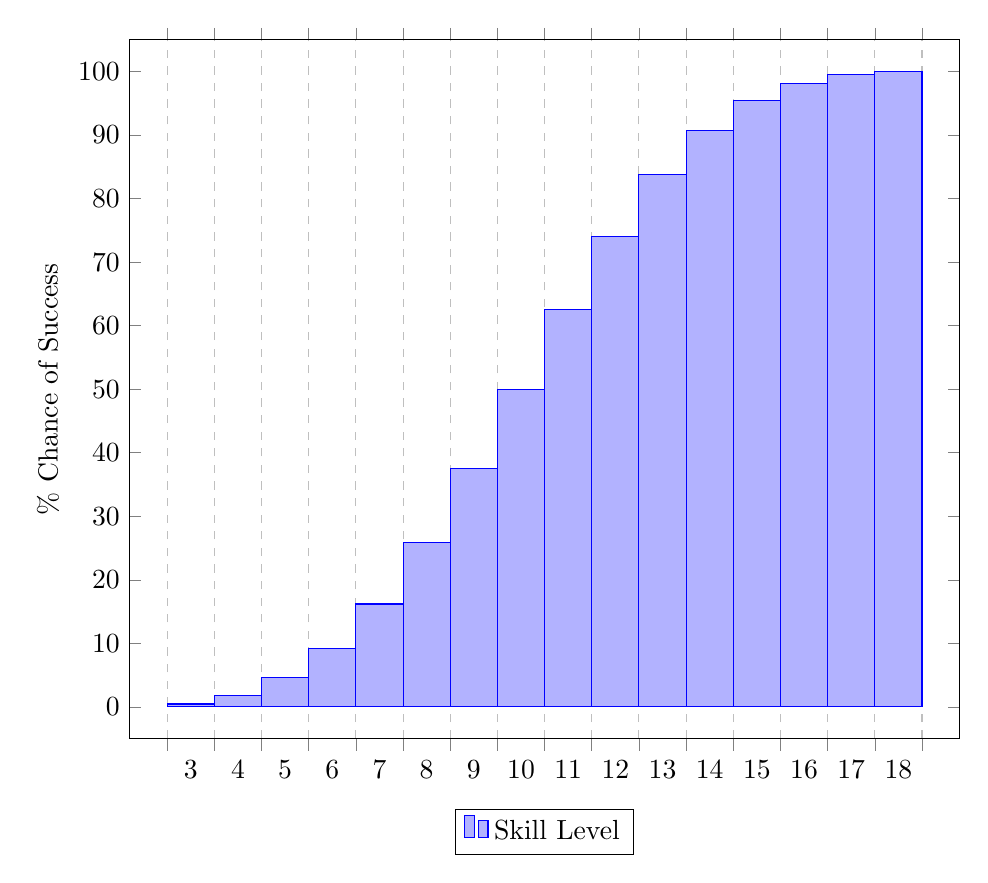
\begin{tikzpicture}
\begin{axis}[
	x tick label style={/pgf/number format/1000 sep=},
	ylabel=\% Chance of Success,
	enlargelimits=0.05,
	ytick = {0, 10, 20, 30, 40, 50, 60, 70, 80, 90, 100},
	legend style = {
	    at={(0.5,-0.1)},
	    grid style = dashed,
	    anchor=north,legend columns=-1
	},
	ybar interval = 1,
]
\addplot 
	coordinates {
	    (3, 0.46) 
	    (4, 1.85)
		(5, 4.63) 
		(6, 9.26) 
		(7, 16.20) 
		(8, 25.93) 
		(9, 37.50) 
		(10, 50.00) 
		(11, 62.50) 
		(12, 74.07)
		(13, 83.80)
		(14, 90.74)
		(15, 95.37)
		(16, 98.15)
		(17, 99.54)
		(18, 100.00)
		(19, 0)
	};
\legend{Skill Level}
\end{axis}
\end{tikzpicture}\\
The graph above shows the probability of succeeding a skill roll.
If your player has an effective skill of 10, they have a 50\% chance of succeeding that roll.
If they have a skill of 12, the chance of success goes up to 74\%.
\end{document}
